\chapter{概率极限}\label{chap:limitation}
\begin{introduction}[考试重点]
    \item 收敛性
    \item Borel-Cantelli引理
    \item 各种概率不等式
    \item 特征函数在处理概率极限定理中的应用
    \item 各种大数定律及证明,如雷尔-康特立引理
    \item 中心极限定理
\end{introduction}
\section{收敛}

\begin{definition}
    若随机变量序列$\left\{ X_n: \Omega \to \mathbb{R} \right\}$与随机变量$X:\Omega \to \mathbb{R}$间存在以下关系:
    \[ \P\left\{ \omega \in \Omega: \lim_{n \to \infty}\abs{ X_n(\omega) - X(\omega)} < \epsilon \right\} =1, \forall \epsilon > 0\]
    则称$X_{n}$\textbf{几乎必然收敛}(converges almost surely)于$X$, 记为$X_{n} \xrightarrow{\as} X$。
\end{definition}

\begin{remark}
    类似于微积分中逐点收敛的条件。考察满足条件$\lim_{n \to \infty}\abs{ X_n(\omega) - X(\omega)} < \epsilon$的样本点,这些样本点组成事件的概率为1。
\end{remark}

% 若
%     \[ \P\{\lim\limits_{n\to\infty}X_{n} \neq X_{\infty}\} = 0
%         \iff \P\{\abs{X_{n}-X_{\infty}}>\e ~~\mathrm{i.o.}\} = 0, \ \forall \e>0 \]
%     \[ \hspace{2.33em} {\color{gray}(\text{利用概率$\P$的连续性})} ~\iff \lim_{N\to\infty}\P(\cup_{n=N}^{\infty}\{\abs{X_{n}-X_{\infty}}>\e\}) = 0, \ \forall \e>0 \]
% 注意$\{A_{n} ~~\mathrm{i.o.}\} = \{\sum_{n=1}^{\infty}\1_{A_{n}} = \infty\} = \bigcap_{N=1}^{\infty}\bigcup_{n=N}^{\infty} A_{n}$表示$A_{n}$发生\emph{无穷多次}(infinitely often). \vspace{0.2ex}


\begin{definition}
    若随机变量序列$\left\{ X_n: \Omega \to \mathbb{R} \right\}$与随机变量$X:\Omega \to \mathbb{R}$间存在以下关系:
    \[ \lim_{n\to\infty}\P\{\omega \in \Omega: \abs{X_n(\omega) - X(\omega)}<\e\} = 1, \ \forall \e>0. \]
    则称$X_{n}$\textbf{依概率收敛}(converges in probability)于$X$, 记为$X_{n} \xrightarrow{\P} X$。
\end{definition}

\begin{remark}
    即对于$Z_i$,事件$A_i=\{\omega \in \Omega: \abs{X_n(\omega) - X(\omega)}<\e\}$,$P(A_i)$将逐渐变为1。
\end{remark}

\begin{figure*}[h]
    \centering
    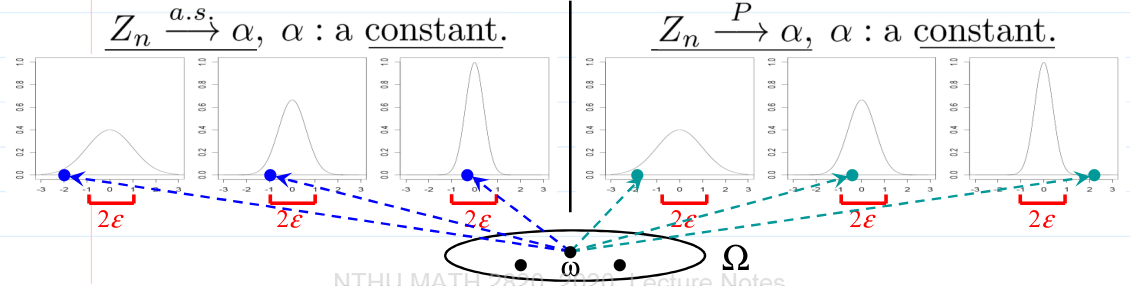
\includegraphics[width=0.9\textwidth]{image/converge1.png}
\end{figure*}

\begin{remark}
    对于几乎必然收敛的情况,每个样本点上的序列随机变量都在逐渐趋近收敛变量;而对于依概率收敛的情况,由于对某个样本点的概率为0(例如连续随机变量),可能某一次样本点的序列随机变量接近收敛变量,下一次又离开收敛变量,只有保证总体概率趋近1即可。
\end{remark}

易见$X_{n} \xrightarrow{\as} X_{\infty} \implies X_{n} \xrightarrow{\P} X_{\infty}$, 但是反之不成立, 例如概率空间$((0,1],\mathscr{B}_{(0,1]},\mathrm{Uniform}((0,1]))$上的\emph{打字机序列}
\[ \xi_{n} = \1_{(n/2^{k}-1,(n+1)/2^{k}-1]}, \quad 2^{k} \le n < 2^{k+1} \]
适合$\P\{\abs{\xi_{n}}>\e\} \le 1/2^{k} \to 0$, 而$\varlimsup \xi_{n} \equiv 1$且$\varliminf \xi_{n} \equiv 0$, 所以$\lim \xi_{n}(\omega)$对$\forall \omega \in (0,1]$都不存在.

\begin{proposition}
    依概率收敛是几乎必然收敛的\underline{必要条件},但\underline{不是充分条件}。
\end{proposition}

\begin{example}
    依概率收敛而不几乎必然收敛的实例:
    设样本空间为$\Omega = (0,1]$,概率均匀分布在样本空间上,即$P([a,b])=b-a,0<a<b<1$。接下来对于$k \in \mathbb{N}_+$,将区间$(0,1]$分为$2^{k}$个等长的子区间,并分别记为$I_{k,j}=(\frac{j-1}{2^k},\frac{j}{2^k}]$。

    按以下方式定义随机变量序列$\left\{ X_n: \Omega \to \mathbb{R} \right\}$:
    \[ X_n(\omega)=\begin{cases}
            1, \omega \in I_{k,j}    \\
            0, \omega \notin I_{k,j} \\
        \end{cases} ,\quad n = 2^k+j-2\]
    同时定义随机变量$X: \Omega \to \mathbb{R}$为$X(\omega)=0,\forall \omega \in \Omega$

    由于对任意$0<\epsilon<1$ 
    \[ \P\{\omega \in \Omega: \abs{X_n(\omega) - X(\omega)}<\e\}=1-\frac{1}{2^K} \to 1  \]
    所以$X_{n} \xrightarrow{\P} X$。
    然而对于任意$\omega \in \Omega$,无论k为何数,此次分割中,总有一个区间包含此样本点。即有无数个$X_i(\omega) = 1$。所以
    \[ \P\left\{ \omega \in \Omega: \lim_{n \to \infty}\abs{ X_n(\omega) - X(\omega)} < \epsilon \right\} =\P\{\emptyset \}=0 \]
    所以$X_{n}$不几乎必然收敛到$X$。
\end{example}

\begin{definition}
    设随机变量 $ X, X_1,  X_2, \dotsc $  的分布函数分别为 $ F (x), F_1 (x), F_2 (x), \dotsc $。若对 $ F (x) $ 的任一\underline{连续点} $x$, 都有
    \[ \lim_{n \to +\infty} F_n (x) = F (x) \]
    则称 $ \{ F_n (x) \} $ \textbf{弱收敛}于 $ F (x) $, 记作    $F_n (x) \xrightarrow{W}{\to} F (x)$;也称 $ \{ X_n \} $ 按\textbf{分布收敛}于$X$,记作$X_n \xrightarrow{d}{\to} X$
\end{definition}

\begin{proposition}
    依分布收敛是依概率收敛的\underline{必要条件},但\underline{不是充分条件}。但若依概率收敛到一个\underline{常数随机变量},则也可推出依分布收敛。
\end{proposition}

\begin{theorem}[连续映射定理]
    设$g: \mathbb{R}^k \mapsto \mathbb{R}$为\underline{连续}函数,则随机向量序列通过次映射后收敛情况与原先相同:
    \begin{align*}
        X_n^{(i)} \xrightarrow{\as} X^{(i)} &\Rightarrow g(X_n^{(1)},\cdots X_n^{(k)}) \xrightarrow{\as} g(X^{(1)},\cdots X^{(k)})\\
        X_n^{(i)} \xrightarrow{\P} X^{(i)} &\Rightarrow g(X_n^{(1)},\cdots X_n^{(k)}) \xrightarrow{\P} g(X^{(1)},\cdots X^{(k)})\\
        (X_n^{(i)}) \xrightarrow{d} (X^{(i)}) &\Rightarrow g(X_n^{(1)},\cdots X_n^{(k)}) \xrightarrow{d} g(X^{(1)},\cdots X^{(k)})\\
    \end{align*}
\end{theorem}
\begin{remark}
    随机向量依分布收敛是指\underline{联合}分布函数收敛。
\end{remark}

\begin{theorem}[Slutsky定理]\label{thm:Slutsky}
    若$X_n \xrightarrow{d} X, Y_n \xrightarrow{P} a$,其中$a$是常数,则:
    \begin{itemize}
        \item $Y_n X_n \xrightarrow{d} a X$
        \item $Y_n + X_n \xrightarrow{d} a + X$
        \item $\frac{X_n}{Y_n}  \xrightarrow{d} \frac{X}{a}$,若对所有的$n$都有$P(Y_n\neq 0)=1$,并且$a\neq 0$
    \end{itemize}
\end{theorem}

\begin{proof}
    由条件可知,$(X_n,Y_n) \xrightarrow{d} (X,a)$,且$g_1(X_n,Y_n)=X_n Y_n, g_2(X_n,Y_n)=X_n+Y_n, g_3(X_n,Y_n)=\frac{X_n}{Y_n}$都是连续函数($g_3$在定理中的限制下),所以仍然保持依分布收敛。
\end{proof}
\begin{remark}
    当$Y_n \xrightarrow{P} a$才能得出$(X_n,Y_n) \xrightarrow{d} (X,a)$;若$Y_n$依分布收敛到其他随机变量,则未必成立。
\end{remark}

\begin{theorem}[theta方法的极限定理]
    设
    \[ \frac{\sqrt{n}(X_n-\theta)}{\sigma} \xrightarrow{d} N(0,1) \]
    那么对于连续函数$g$,若$g'(\theta)\neq 0$存在,则
    \[ \frac{\sqrt{n}(g(X_n)-g(\theta))}{\sigma|g'(\theta)|} \xrightarrow{d} N(0,1) \]
\end{theorem}

\begin{proof}
    %TODO
\end{proof}

\begin{theorem}[连续性定理]\label{thm:continuity}
    设$F_n(x)$是一个累计函数序列,并且分别对应矩母函数$M_n(t)$;$F(x)$是一个累计函数,并且对应矩母函数$M(t)$。那么,
    \[ \forall t \in U(0,\delta) ,s.t. \lim_{n \to \infty}M_n(t) = M(t)\]
    是在$F(x)$的所有连续点上$F_n(x) \xrightarrow{M} F(x)$的充要条件。
\end{theorem}
\begin{remark}
    若矩母函数不存在,替换成特征函数,定理也成立。但是,不能替换成密度函数或质量函数
\end{remark}

\begin{example}
    离散情况:\\
    设均匀随机变量$X_n \sim U(-\frac{1}{2},\frac{1}{2})$,那么$X_n \xrightarrow{d} 0$。然而$P_n(x) \to 0, \forall x \in \mathbb{R}$(不满足质量函数定义),并且$\lim_{n \to \infty}F_n(0)=\frac{1}{2}$(不满足累积函数定义)

    连续情况:\\
    设累积函数为$F_n(x)=x-\frac{\sin (2n\pi x)}{2n\pi}, 0<x<1$,那么$F_n \xrightarrow{d} U(0,1)$。然而$f_n(x)$无极限
\end{example}

\begin{example}[泊松分布收敛于正态分布]
    令$X_n \sim P(\lambda_n)$,并且$\lim_{n \to \infty}\lambda_n =\infty$。将变量标准化:
    \[ Z_n=\frac{X_n-\lambda_n}{\sqrt{\lambda_n}} \]
    那么
    \[M_{Z_n}(t)=\ee^{-t\sqrt{\lambda_n}}M_{X_n}(t)(\frac{t}{\sqrt{\lambda_n}})=\exp (-t\sqrt{\lambda_n}+\lambda_n(e^{\frac{t}{\sqrt{\lambda_n}}-1}))\]
    由于
    \[ \lim_{n \to \infty}\ln (M_{Z_n}(t))=\lim_{\lambda_n \to \infty}-t\sqrt{\lambda_n}+\lambda_n(e^{\frac{t}{\sqrt{\lambda_n}}-1})=\frac{t^2}{2} \]
    所以$Z_n \xrightarrow{d} N(0,1)$,即若$\lambda$很大,可通过$N(\lambda,\lambda)$估计$P(\lambda)$
\end{example}

\section{大数定理}

\begin{theorem}[弱大数定理]
    设随机变量$X_1,\cdots ,X_n$相互独立,且$E(X_i)=\mu,\operatorname{Var}(X_i)=\sigma^2$,那么
    \[ \overline{X_n}=\frac{1}{n}\sum_{i=1}^n X_i \xrightarrow{\P} \mu \]
\end{theorem}

\begin{remark}
    柯西分布无均值、方差,不能使用此定理。
\end{remark}

\begin{proof}
    易知
    \[ E(\overline{X_n})=\mu,\operatorname{Var}(\overline{X_n})=\frac{\sigma^2}{n} \]
    再通过切比雪夫不等式有:
    \[ P(\left\vert \overline{X_n}-\mu \right\vert >\epsilon)<\frac{\operatorname{Var}(\overline{X_n})}{\epsilon^{2}}=\frac{\sigma^2}{n \epsilon^2} \to 0 \]
\end{proof}

\begin{theorem}[强大数定理]
    设随机变量$X_1,\cdots ,X_n$相互独立,且$E(X_i)=\mu,\operatorname{Var}(X_i)=\sigma^2$,那么
    \[ \overline{X_n}=\frac{1}{n}\sum_{i=1}^n X_i \xrightarrow{\as} \mu \]
\end{theorem}

\begin{example}[蒙特卡洛积分]
    为计算积分$I(f)=\int_0^1 f(x)\mathrm{d}x$,生成随机数$X_1,\cdots ,X_n \operatorname{i.i.d.} \sim U(0,1)$,并且计算$\hat{I}(f)=\overline{Y_n}, Y_i=f(X_n) $。由于$X_1,\cdots ,X_n \operatorname{i.i.d.}$,所以$Y_1,\cdots ,Y_n \operatorname{i.i.d.}$;并且$E(Y_i)=E(f(X_i))=\int_0^1 f(x)\cdot 1\mathrm{d}x=I(f)$,所以$\hat{I}(f)\xrightarrow{\P} E(Y_i)=I(f)$
\end{example}

\begin{example}[样本方差]\label{ex:sample_var}
    设随机变量$X_1,\cdots ,X_n \operatorname{i.i.d.}$,并且均值和方差分别为$\mu,\sigma$。令:
    \[ S_n^2=\frac{1}{n}\sum_{i=1}^n(X_i-\overline{X_n}) = (\frac{1}{n}\sum_{i=1}^nX_i^2)-\overline{X_n}^2 +\]
    由于$g(x)=x^2$是连续函数,所以$\overline{X_n}^2 \xrightarrow{\P} \mu^2$。由于$X_1^2,\cdots X_n^2 \operatorname{i.i.d.}$,且$E(X_i^2)=\sigma^2+\mu^2$,所以$\overline{X_n^2} \xrightarrow{\P} \mu^2+\sigma^2$。因此:
    \[ S_n^2 \xrightarrow{\P}\mu^2+\sigma^2-\mu^2= \sigma^2 \]
\end{example}

\begin{example}\label{ex:t_disc_to_normal}
    若$X_n \sim t_n$,则$X_n \xrightarrow{d} N(0,1)$。
    令$Z \sim N(0,1),U_1,\cdots ,U_n \sim \chi^2_1$相互独立,则$\frac{Z}{\sqrt{(U_1+\cdots+U_n)/n}} \sim t_n$。由于$E(U_i)=1$,所以$\overline{U_n} \xrightarrow{\P} 1$,所以$\sqrt{\overline{U_n}} \xrightarrow{\P} 1$,所以$t_n=\frac{Z}{\sqrt{\overline{U_n}}} \xrightarrow{d} N(0,1)$(定理\ref{thm:Slutsky})。
\end{example}

\begin{example}
    若$X_n \sim F_{m,n}$,则$mX_n \xrightarrow{d} \chi^2_m$。
    令$U \sim \chi^2_m,V_1,\cdots ,V_n \sim \chi^2_1$相互独立,则$\frac{U/m}{(V_1+\cdots+V_n)/n} \sim F_{m,n}$。由于$E(V_i)=1$,所以$\overline{V_n} \xrightarrow{\P} 1$,所以$mF_{m,n}=\frac{U}{\overline{V_n}} \xrightarrow{d} \chi^2_m$(定理\ref{thm:Slutsky})。
\end{example}

\section{中央极限定理}

\begin{theorem}[中央极限定理]\label{thm:central_limit}
    设随机变量$X_1,\cdots ,X_n,\operatorname{i.i.d.}$,且$E(X_i)=\mu,\operatorname{Var}(X_i)=\sigma^2$,令
    \[ \overline{X_n} = \frac{1}{n}\sum_{i=1}^n X_i, T_n=\sum_{i=1}^n X_i\]
    则:
    \[ \lim_{n \to \infty}P(\frac{T_n-n \mu}{\sigma\sqrt{n}}\le x)=\lim_{n \to \infty}P(\frac{\sqrt{n}(\overline{X_n}-\mu)}{\sigma}\le x) =\Phi(x)\]
    其中$\Phi(x)$是$N(0,1)$的累积函数,即:
    \[ \frac{T_n-n \mu}{\sigma\sqrt{n}}=\frac{\sqrt{n}(\overline{X_n}-\mu)}{\sigma} \xrightarrow{d} N(0,1)\]
\end{theorem}

\begin{proof}
    令$W_i=\frac{X_i-\mu}{\sigma}$,则$E(W_i)=0,\operatorname{Var}(W_i)=1$。再令$Z_n=\frac{T_n-n \mu}{\sigma\sqrt{n}}=\frac{1}{\sqrt{n}}\sum_{i=1}^n W_i$。则
    \begin{align*}
        M_{Z_n}(t) &= \left[ M_{W}(\frac{t}{\sqrt{n}}) \right]^n \\
        &= \left[ M_{W}(0)+M_{W}'(0)\frac{t}{\sqrt{n}}+\frac{M_{W}''(0)}{2}(\frac{t}{\sqrt{n}})^2 +o(\frac{1}{n}) \right]^n \\
        &= \left[ 1 + \frac{t^2}{2n}+ o(\frac{1}{n}) \right]^n\\
        & \to e^{\frac{t^2}{2}}
    \end{align*}
    根据定理\ref{thm:continuity},$Z_n \xrightarrow{d} N(0,1)$。
\end{proof}
\begin{remark}
    若矩母函数不存在,可替换为特征函数。
\end{remark}

\begin{example}[二项分布近似为正态分布]
    若随机变量$X_1,\cdots ,X_n \operatorname{i.i.d.} \sim B(1,p)$, 则$T_n \sim B(n,p)$. 其中$E(T_n)=nE_(X_i)=np, \operatorname{Var}(T_n)=n\operatorname{Var}(X_i)=np(1-p)$. 根据中央极限定理有:
    \[ \frac{T_n - np}{\sqrt{np(1-p)}} \xrightarrow{d} N(0,1) \]
    即当n很大时, $B(n,p)$可用$N(np,np(1-p))$近似.
\end{example}
\begin{remark}
    其他与二项分布一样, 可以通过独立同分布的随机变量相加得到的分布,也可在一定条件下近似为正态分布. 例如Gamma分布(可通过指数分布相加得到), 泊松分布(泊松分布相加), 负二项分布(几何分布相加), 参见图\ref{fig:relationship_among_univariate_distributions}
\end{remark}
\begin{remark}
    由定理\ref{thm:Poisson_theorem}可知, 当$B(n,p)$中$n$很大$p$很小时, 二项分布可近似为泊松分布; 而泊松分布$\lambda$很大时, 又可近似为正态分布.
\end{remark}

\begin{example}[测量误差估计]
    假设每次测量结果为独立同分布的随机变量$X_1,\cdots ,X_n$, 其均值与方差分别为$\mu,\sigma^2$. 由中央极限定理可知$\frac{\sqrt{n}(\overline{X_n}-\mu)}{\sigma} \xrightarrow{d} N(0,1)$. 由例\ref{ex:sample_var}可知$S_n^2 \xrightarrow{\P} \sigma^2$, 即$\frac{\sigma}{S_n} \xrightarrow{\P} 1$(定理\ref{thm:Slutsky}). 所以:
    \[ \frac{\sqrt{n}(\overline{X_n}-\mu)}{S_n}=\frac{\sqrt{n}(\overline{X_n}-\mu)}{\sigma}\frac{\sigma}{S_n} \xrightarrow{d} N(0,1)\cdot 1=N(0,1) \]
    即可以通过分布$N(0,\frac{S_n^2}{n})$估计测量误差$\overline{X_n}-\mu$
\end{example}
\begin{remark}
    由定理\ref{thm:normal_sample_mean_variance}可知$\frac{\sqrt{n}(\overline{X_n}-\mu)}{S_n} \sim t_{n-1}$. 但由例\ref{ex:t_disc_to_normal}可知, $n\to \infty$时, $t$分布收敛于正态分布, 所以不冲突.
\end{remark}